\documentclass{exam}

%....................................
% PACOTES USADOS
%....................................

\usepackage[portuguese]{babel}
\usepackage[utf8]{inputenc}
\usepackage{geometry}
\usepackage[list-final-separator={ e }, output-decimal-marker={,}]{siunitx}
\usepackage{graphicx}
\usepackage{float}
\usepackage{verbatim}
\usepackage{lmodern}
\usepackage{xpatch}
\usepackage{enumerate}
\usepackage{enumitem}
\usepackage{multicol, setspace}
\usepackage{indentfirst}
\usepackage{parskip}
\usepackage{amssymb, amsmath, amsfonts, dsfont}
\usepackage{makeidx}
\usepackage[sharp]{easylist}
\usepackage[pdftex]{hyperref}

%\usepackage{textcomp}

%....................................
% OUTRAS CONFIGURAÇÕES
%....................................


\pagestyle{headandfoot}

%\runningfootrule

\firstpageheader{\texttt{spholima@gmail.com}}{}{
\includegraphics[scale=.9]{by-nc-sa}}
\runningheader{\textsc{Números inteiros}}{}{
\includegraphics[scale=.9]{by-nc-sa}}
\firstpagefooter{}
	{\textsc{\thepage}}
	{}
\runningfooter{}
	{\textsc{\thepage}}
	{}

\geometry{a4paper,
	top=2.5cm,
	bottom=2.5cm,
	left=1.5cm,
	right=1.5cm
}
\columnsep=0.8cm

%....................................
% CONFIGURAÇÕES DA CLASSE EXAM
%....................................
\renewcommand{\thequestion}{\bf \arabic{question}}
\renewcommand{\choicelabel}{{\bf (\thechoice)}}
\pointpoints{ponto}{pontos}
\pointformat{[\bf \thepoints]}



%....................................
% INÍCIO DO DOCUMENTO
%....................................

\begin{document}

	\begin{center}
\large{\textsc{Tópico 01 - Lista 02 - Números inteiros\\
Março de 2020\\ (em plena crise do corona vírus$\ldots$)}}
	\end{center}

%\maketitle
	
	\begin{multicols*}{2}
	\setlength{\columnseprule}{1pt}


\tableofcontents

\section{Momento netflix}

	\begin{itemize}
	
	\item Representação na reta e interpretações: \url{https://youtu.be/fmiw3ksXOmk}
	
	\item Subtração de inteiros: \url{https://youtu.be/P3YIiKk0d-M?t=385}
		
	\end{itemize}


\section{Representação na reta numérica}

O conjunto dos inteiros, $\mathbb{Z}$, pode ser representado graficamente em uma reta numérica, centrada no número zero (origem da reta numérica) e que cresce indefinidamente para a direita (números negativos) e para a esquerda (números positivos).

\begin{figure}[H]
	\centering
	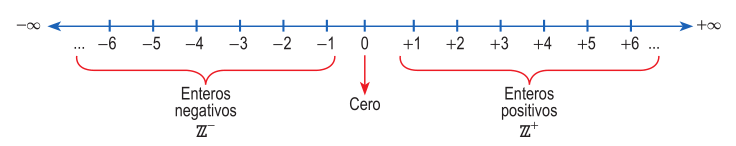
\includegraphics[scale=0.45]{fig01}
	\caption{Representação dos inteiros na reta.}
	\label{fig:retaNumerica}
\end{figure}

	\subsection{Outras notações}
	
	\begin{itemize}
	
	\item O conjunto dos números \textit{inteiros não negativos} é denotado por $\mathbb{Z_+}$:
	
	\[ \mathbb{Z_+} = \{0,\, 1,\, 2,\, 3,\, \ldots\} \]
	
	\item O conjunto dos números \textit{inteiros não positivos} é denotado por $\mathbb{Z_-}$:
	
	\[ \mathbb{Z_-} = \{\ldots, \, -3,\, -2,\, -1,\, 0 \} \]
	
	\end{itemize}


\section{Comparação de inteiros}

Dados dois números inteiros diferentes, o maior deles estará sempre mais à direita na reta numérica.


\begin{figure}[H]
	\centering
	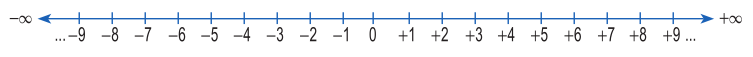
\includegraphics[scale=0.44]{fig02}
	\caption{Representação dos inteiros na reta.}
	\label{fig:retaNumerica2}
\end{figure}

		\textbf{Exemplos:}

\begin{easylist}[enumerate]
	
	## $+4$ está à direita de $+1$, então $+1 < +4$.
	## $+5$ está à direita de $-3$, então $-3 < +5$.
	## $-4$ está à direita de $-9$, então $-9 < -4$.
	## $0$ está à direita de $-7$, então $-7 < 0$.
	
\end{easylist}

	\subsection{Subtração de inteiros}

		\subsubsection{Módulo (ou valor absoluto)}
		
		O valor absoluto de um número inteiro, denotado por $|a|$, nada mais é do que o próprio número sem o sinal.
		Dessa forma, temos que o módulo de um número positivo é ele próprio; e o módulo de um número negativo é o próprio número, porém com o sinal invertido (positivo).
		
		\textbf{Exemplos:}
		
		\begin{easylist}[enumerate]
			## O módulo de $-20$ é $20$.
			## O módulo de $35$ é $35$.
			## O módulo de $-37$ é $37$.
			## O módulo de $0$ é $0$.
			## $|5| = 5$
			## $|-4| = -(-4) = 4$
			## $|-12| = -(-12) = 12$
			## $|0| = 0$
						
		\end{easylist}
		
		O módulo de um número é interpretado geometricamente como sendo a distância do número à origem da reta numérica.
		

		\subsubsection{Simétrico (ou oposto)}
		
		Dois números inteiros são \textit{simétricos} (ou \textit{opostos})  quando possuem o mesmo valor absoluto, mas com sinais diferentes.
		
		\textbf{Exemplos:}
		
		\begin{easylist}[enumerate]
			## $-3$ é o oposto de $+3$.
			## $+4$ é o oposto de $-4$.
			## O simétrico de $0$ é $0$.
				
		\end{easylist}

Utilizando o conceito de simetria, podemos definir a operação de subtração como:

\textbf{\textit{Subtrair um número é a mesma coisa que somar com o seu simétrico. Ou seja, basta transformar a operação em adição e inverter o sinal do segundo número.}}

		\textbf{Exemplos:}

		\begin{easylist}[enumerate]
		
			## $8 - 5 = 8 + (-5) = 3$
			## $4 - 6 = 4 + (-6) = -2$
			## $8 - (-3) = 8 + (3) = 11$
			## $(-5) - (-11) = (-5) + (+11) = 6$
			## $-2-7 = (-2) + (-7) = -9$
			
			
		\end{easylist}

\begin{questions}

	\qformat{\textbf{Questão} \thequestion \dotfill}

\section{Questões para treinamento}

\question Efetuas as operações a seguir:
	\begin{choices}

		\choice $(-3)-(-6)=$
		\choice $(-3)-(-5)=$
		\choice $(+5)-(+3)=$
		\choice $(-5)-(-4)=$
		\choice $(+16)-(+12)=$
		\choice $(-21)-(-4)=$
		\choice $(-13)-(-13)=$
		\choice $(-32)-(-14)=$
		\choice $(+7)-(+9)=$
		\choice $(-16)-(-22)=$
		\choice $(-3)-(-24)=$
		\choice $(+7)-(+3)=$
		\choice $(-26)-(-19)=$
		\choice $(-29)-(-33)=$
		\choice $(+3)-(+4)=$
		\choice $(-21)-(-11)=$
		\choice $(+34)-(+42)=$
		\choice $(-55)-(-20)=$
		\choice $(+60)-(+30)=$
		\choice $(-7)-(-18)=$

	\end{choices}

	\question Mais exercícios.

\begin{choices}
	
	\choice $(-7)-(+3)=$
	\choice $(+3)-(-9)=$
	\choice $(+4)-(-4)=$
	\choice $(+8)-(-11)=$
	\choice $(+15)-(-19)=$
	\choice $(+15)-(-9)=$
	\choice $(-18)-(+26)=$
	\choice $(-23)-(+15)=$
	\choice $(+13)-(-7)=$
	\choice $(+16)-(-14)=$
	\choice $(+8)-(-21)=$
	\choice $(+4)-(-5)=$
	\choice $(-34)-(+18)=$
	\choice $(+32)-(-42)=$
	\choice $(-22)-(+5)=$
	\choice $(+45)-(-18)=$
	\choice $(+38)-(-40)=$
	\choice $(-63)-(+32)=$
	\choice $(+72)-(-33)=$
	\choice $(-16)-(-24)=$
	
\end{choices}

\question Mais exercícios: subtração de inteiros.

\begin{choices}
	
	\choice $(-2)-(-5)=$
	\choice $(-4)-(-2)=$
	\choice $(+5)-(+4)=$
	\choice $(-3)-(-4)=$
	\choice $+6 - (+12)=$
	\choice $(-26)-(-3)=$
	\choice $(-14)-(-31)=$
	\choice $(-35)-(-21)=$
	\choice $+5 - 8=$
	\choice $(-15)-(-18)=$
	\choice $(-2)-(-26)=$
	\choice $+6 - 9=$
	\choice $-28 - (-17)=$
	\choice $(-19) - (-36)=$
	\choice $(+6) - 3=$
	\choice $-12 - (-13)=$
	\choice $+32 - 22=$
	\choice $-45 - (-10)=$
	\choice $40 - 30=$
	\choice $(-9) - (-29)=$
	
\end{choices}


\question Mais exercícios.

\begin{choices}
	
	\choice $-22 - 62=$
	\choice $-19 - (-25)=$
	\choice $44 - (-33)=$
	\choice $-18 - 21=$
	\choice $-33 - (-18)=$
	\choice $25 - (-13)=$
	\choice $-32 - 51=$
	\choice $-16 - (-27)=$
	\choice $-9 - 13=$
	\choice $-24 - (-50)=$
	\choice $25 - (-52)=$
	\choice $-31 - (-23)=$
	\choice $-42 - (-20)=$
	\choice $73 - (-54)=$
	\choice $28 - 15=$
	\choice $65 - (-12)=$
	\choice $37 - (-75)=$
	\choice $-76 - (-48)=$
	\choice $-20 - (-17)=$
	\choice $39 - (-28)=$
	
\end{choices}


\question Mais exercícios de subtração.

\begin{choices}
	
	\choice $-23 - 46=$
	\choice $-12 - (-15)=$
	\choice $51 - (-42)=$
	\choice $-15 - 15=$
	\choice $-27 - (-12)=$
	\choice $35 - (-17)=$
	\choice $-47 - 36=$
	\choice $-21 - (-26)=$
	\choice $-4 - 8=$
	\choice $-12 - (-27)=$
	\choice $15 - (-35)=$
	\choice $-17 - (-11)=$
	\choice $-25 - (-13)=$
	\choice $98 - (-64)=$
	\choice $17 - 41=$
	\choice $52 - (-67)=$
	\choice $13 - (-36)=$
	\choice $-82 - (-10)=$
	\choice $-70 - (-22)=$
	\choice $16 - (-37)=$
	
\end{choices}

\section{Problemas}
	
	Se for, vá na paz.

\question Rubens nasceu no ano 92 a.C. e se casou aos 29 anos de idade. Em que ano ele se casou?

\question Se um termômetro marca \SI{9}{\celsius} depois que a temperatura subiu \SI{17}{\celsius}, qual era a temperatura inicial?

\question Um balão subiu 17 quilômetros e, em seguida, desceu 9 quilômetros. A quantos quilômetros o balão se encontra do ponto que ele saiu?

\question Um helicóptero que voa a 510 metros acima do nível do mar, identifica um submarino que se encontra a uma profundidade de 203 metros. A que distância se encontra o submarino do helicóptero?

\question De um depósito, que contém 800 litros de água, se retiram 240 litros e, logo após, acrescentam 250 litros. Depois, se retiram 180 litros e acrescentam $x$ litros. Qual é o valor de $x$ se ao final o depósito contém 500 litros de água?

\question Hélder e Laura partem de um mesmo lugar de bicicleta. Hélder avança 7 quilômetros e logo retrocede 2 quilômetros. Já Laura, avança 7 quilômetros e retrocede 1. Ao final, a que distância se encontra um do outro?

\question Em uma cidade ao norte da Rússia, a temperatura interna de uma casa é \SI{18}{\celsius}. Em um dado instante, a temperatura ambiente externa era de \SI{12}{\celsius} negativos. Ao sair do interior para o exterior dessa casa, qual é a variação de temperatura que uma pessoa experimenta?

\question Quantos anos foram transcorridos entre 520 a.C. e 450 a.C.?

\question O planeta Vênus é um dos mais quentes do nosso sistema solar, tendo uma temperatura média de \SI{450}{\celsius}. Enquanto isso, seu amigo Plutão é um dos mais frio, com temperaturas médias de \SI{250}{\celsius} negativos. Quantos graus Plutão é mais frio que Vênus?


\question No deserto de Gobi, localizado na Ásia, podem ser verificadas diferenças de temperatura de até \SI{60}{\celsius} entre o dia e a noite. Durante o dia, a temperatura chega a \SI{50}{\celsius}. A quanto chega a temperatura à noite?


\question Um avião levantou voo de uma cidade A que está a 50 metros acima do nível do mar. Subiu 300 metros, depois desceu 40 metros, subiu mais 80 metros, desceu até a metade da altura que estava, em relação ao nível do mar, então subiu mais 100 metros. Quanto precisará agora descer para chegar ao chão da cidade B, localizada a 30 metros acima do nível do mar?

\question O isolamento térmico de um avião permite suportar diferenças de temperatura de até \SI{60}{\degree C} seu interior e seu exterior. Mantendo a temperatura interna do avião em \SI{18}{\degree C}, qual é a mínima temperatura externa suportada?


\end{questions}

	\end{multicols*}


\newpage
\section{Gabarito}

\begin{multicols*}{4}
\setlength{\columnseprule}{1pt}
\begin{enumerate}

\item 	a) $3$ \\
		b) $2$ \\
		c) $3$ \\
		d) $-1$ \\
		e) $4$ \\
		f) $-17$ \\
		g) $0$ \\
		h) $-18$ \\
		i) $-2$ \\
		j) $6$ \\
		k) $21$ \\
		l) $4$ \\
		m) $-7$ \\
		n) $4$ \\
		o) $-1$ \\
		p) $-10$ \\
		q) $-8$ \\
		r) $-35$ \\
		s) $30$ \\
		t) $11$ \\
		
\item 	a) $-10$ \\
		b) $12$ \\
		c) $8$ \\
		d) $19$ \\
		e) $34$ \\
		f) $24$ \\
		g) $-44$ \\
		h) $-38$ \\
		i) $20$ \\
		j) $30$ \\
		k) $29$ \\
		l) $9$ \\
		m) $-52$ \\
		n) $74$ \\
		o) $-27$ \\
		p) $63$ \\
		q) $78$ \\
		r) $-95$ \\
		s) $105$ \\
		t) $8$ \\

\item 	a) $3$ \\
		b) $-2$ \\
		c) $1$ \\
		d) $1$ \\
		e) $-6$ \\
		f) $-23$ \\
		g) $17$ \\
		h) $-14$ \\
		i) $-3$ \\
		j) $3$ \\
		k) $24$ \\
		l) $-3$ \\
		m) $-11$ \\
		n) $17$ \\
		o) $3$ \\
		p) $1$ \\
		q) $10$ \\
		r) $-35$ \\
		s) $10$ \\
		t) $20$ \\

\item 	a) $-84$ \\
		b) $6$ \\
		c) $77$ \\
		d) $-39$ \\
		e) $-15$ \\
		f) $38$ \\
		g) $-83$ \\
		h) $11$ \\
		i) $-22$ \\
		j) $26$ \\
		k) $77$ \\
		l) $-8$ \\
		m) $-226$ \\
		n) $127$ \\
		o) $13$ \\
		p) $77$ \\
		q) $112$ \\
		r) $-28$ \\
		s) $-3$ \\
		t) $67$ \\


\item 	a) $-69$ \\
		b) $3$ \\
		c) $93$ \\
		d) $-30$ \\
		e) $-15$ \\
		f) $52$ \\
		g) $-83$ \\
		h) $5$ \\
		i) $-12$ \\
		j) $15$ \\
		k) $50$ \\
		l) $-6$ \\
		m) $-12$ \\
		n) $162$ \\
		o) $-24$ \\
		p) $119$ \\
		q) $49$ \\
		r) $-72$ \\
		s) $-48$ \\
		t) $53$ \\

\item 63 a.C.
\item \SI{-8}{\celsius}
\item 8 quilômetros
\item 713 metros
\item 670 litros
\item 1 quilômetro
\item \SI{-30}{\celsius}
\item 70 anos
\item \SI{700}{\celsius}
\item \SI{-10}{\celsius}
\item 265 metros
\item \SI{-42}{\celsius}


\end{enumerate}

\end{multicols*}



\end{document}